\documentclass[{../../master}]{subfiles}
\graphicspath{{../../}}  % 個別コンパイル時の画像パスを解決する

\begin{document}

\section{GMappingのアルゴリズムの概要}
\label{sec:gmapping_algorithm}

GMappingは格子ベースの地図を扱うベイズフィルタ系のSLAMアルゴリズムです.
FastSLAM2.0のアプローチを採用しており,スキャンマッチングによってオドメトリを修正することにより,少ないパーティクルでも良好な推定を行うことができるのが特徴です.

\subsection{GMappingが扱う問題}

\subsubsection{求める解}

ロボットの初期姿勢$\bm{x}_{0}$,観測の時系列リスト$z_{1:t}$,オドメトリ情報$u_{1:t}$が得られたとき,ロボットの軌跡$\bm{x}_{1:t}$と地図$m$の結合確率分布を求めます.
\footnote{論文\cite{Gmapping}に書かれている数式と少し異なりますが,表している事象は同じです.}

\begin{equation}
  p(\bm{x_{1:t}}, m \mid \bm{x}_{0}, z_{1:t}, u_{1:t})
  \label{eq:target_distribution}
\end{equation}

ここで,$\bm{x}_{t}$はロボットの姿勢(Pose)を表すベクトルであり,$\bm{x}_{x} = (x_{t}, y_{t}, \theta_{t})^T$です.
$z_{t}$は時刻$t$で得られた観測の情報で,GMappingではスキャンデータが用いられます.
$u_{t}$は,時刻$t-1$から時刻$t$までにロボットが移動した距離を,ホイールオドメトリで求めた情報です.
また,$1:t$の表記は時刻$1$から時刻$t$までの時系列のリストを表しています.

SLAMの目的は式\ref{eq:target_distribution}の確率分布を求めることにあります.
確率分布を求めることができれば,確率密度が一番高いところにロボットがいるのが尤もらしいと言えるため,結果的にロボットの姿勢を求めることに繋がります.

しかし,式\ref{eq:target_distribution}の確率分布がどのような形状をしているのかは誰にもわかりません.
従って,式\ref{eq:target_distribution}を直接求めることはほぼ不可能に近い難問になります.
そのため,何らかの近似や仮定を用いることによって確率分布を求めることになります.
その近似手法の1つが,GMappingでも用いられているパーティクルフィルタです.

パーティクルフィルタは連続な関数である確率分布を,重みを持ったパーティクルの集合として離散的に近似する手法です.
確率分布の内の確率密度が高い部分が,重みの大きいパーティクルに対応します.
パーティクルの数を無限大に近づけると元の確率分布に近づきます.

% TODO: パーティクルフィルタの概要の説明.1次元のグラフかなんかを書いて説明する

GMappingではRao-Blackwellizationと呼ばれる因数分解を適用して,式\ref{eq:target_distribution}の確率分布を分解しています.

\begin{equation}
  \begin{split}
    &p(\bm{x_{1:t}}, m \mid \bm{x}_{0}, z_{1:t}, u_{1:t}) \\
    &= p(m \mid \bm{x}_{1:t}, \bm{x}_{0}, u_{1:t}, z_{1:t}) \cdot p(\bm{x}_{1:t} \mid \bm{x}_{0}, u_{1:t}, z_{1:t}) \\
    &= p(m \mid \bm{x}_{0:t}, z_{1:t}) \cdot p(\bm{x}_{1:t} \mid z_{1:t}, u_{1:t})
  \end{split}
  \label{eq:rao_blackwellized_distribution}
\end{equation}

式\ref{eq:target_distribution}にRao-Blackwellizationを適用したのが式\ref{eq:rao_blackwellized_distribution}です.
式\ref{eq:rao_blackwellized_distribution}を見ると,この問題はロボットの姿勢の分布$p(\bm{x}_{1:t} \mid z_{1:t}, u_{1:t})$を求める問題と,地図$p(m \mid \bm{x}_{0:t}, z_{1:t})$を求める問題に分解して考えられるようになります.

\subsubsection{SLAMにおける用語}

式\ref{eq:target_distribution}で示すような,SLAMで求める確率分布を「目標分布」または「信念(信念分布)」と呼びます.\cite{上田2019}
パーティクルフィルタを含むベイズフィルタの演算は単純なもので,まずロボットの移動の情報をもとに時刻$t-1$の信念分布を遷移させ,その後センサ等の観測情報を用いて時刻$t$の信念を確定させる,という処理を繰り返します.

ロボットの移動の情報をもとに信念分布を遷移させるときに使う確率モデルを「移動モデル」\cite{thrun2005probabilistic}もしくは「状態遷移モデル」\cite{上田2019}と呼びます.
状態遷移モデルはロボットの移動に含まれるノイズやバイアスを確率的に扱うモデルで,式\ref{eq:motion_model}で表されます.
また,状態遷移モデルによって遷移させられた信念分布を「提案分布」もしくは「事前分布」と呼びます.
Probabilistic Roboticsでは,状態遷移モデルの種類として速度動作モデル(\textsf{motion\_model\_velocity})とオドメトリ動作モデル(\textsf{motion\_model\_odometry})が紹介されています.

\begin{equation}
  p(\bm{x}_{t} \mid \bm{x}_{t-1}, u_{t})
  \label{eq:motion_model}
\end{equation}

状態遷移モデルによって信念分布を遷移した後,観測情報を用いて時刻$t$の信念分布を確定させる際に使う確率モデルを「計測モデル」\cite{thrun2005probabilistic}「観測モデル」\cite{上田2019}と呼びます.
観測モデルは式\ref{eq:measurement_model}で表されます.
提案分布に観測モデルを適用してできた分布を「目標分布」もしくは「事後分布」と呼びます.
Probabilistic Roboticsでは,LiDAR等のレーザーセンサのための観測モデルの種類としてビームモデル(\textsf{beam\_range\_finder\_model})と尤度場モデル(\textsf{likelihood\_field\_model})が紹介されています.

\begin{equation}
  p(z_{t} \mid \bm{x}_{t}, m)
  \label{eq:measurement_model}
\end{equation}

\subsection{問題の定式化}

パーティクルフィルタにおいて,$i$番目のパーティクルの重み$w^{(i)}$は式\ref{eq:particle_weight_equation}で更新されます.

\begin{equation}
  w^{(i)} = \frac{p(\bm{x}_{1:t}^{(i)} \mid z_{1:t}, u_{1:t})}{\pi(\bm{x}_{1:t}^{(i)} \mid z_{1:t}, u_{1:t})}
  \label{eq:particle_weight_equation}
\end{equation}

式\ref{eq:particle_weight_equation}右辺の分子は事後分布,分母は提案分布です.
事後分布と提案分布の差が小さい程フィルタの性能は上がりますが,提案分布$\pi$が事後分布と一致することはまずありません.
また,式\ref{eq:particle_weight_equation}のままだと新しい観測が得られる度に各パーティクルの軌跡の重みを評価しなければならないため,時間が経過するにつれて計算負荷は増大していってしまいます.
ここで,提案分布が式\ref{eq:proposal_assumption}に従うと仮定します.

\begin{equation}
  \pi(\bm{x}_{1:t} \mid z_{1:t}, u_{1:t}) = \pi(\bm{x}_{t} \mid \bm{x}_{1:t-1}, z_{1:t}, u_{1:t}) \cdot \pi(\bm{x}_{1:t-1} \mid z_{1:t-1}, u_{1:t-1})
  \label{eq:proposal_assumption}
\end{equation}

式\ref{eq:proposal_assumption}を使って式\ref{eq:particle_weight_equation}を逐次式に変換すると,

\begin{equation}
  \begin{split}
    &w^{(i)} = \frac{p(\bm{x}_{1:t}^{(i)} \mid z_{1:t}, u_{1:t})}{\pi(\bm{x}_{1:t}^{(i)} \mid z_{1:t}, u_{1:t})} \\
    &= \eta \frac{p(z_{1:t} \mid \bm{x}_{1:t}^{(i)}, z_{1:t-1}) p(\bm{x}_{t}^{(i)} \mid \bm{x}_{t-1}^{(i)}, u_{t})}{\pi(\bm{x}_{t}^{(i)} \mid \bm{x}_{1:t-1}^{(i)}, z_{1:t}, u_{1:t})} \cdot \frac{p(\bm{x}_{1:t-1}^{(i)} \mid z_{1:t-1}, u_{1:t-1})}{\pi(\bm{x}_{1:t-1}^{(i)} \mid z_{1:t-1}, u_{1:t-1})} \\
    &= \eta \frac{p(z_{1:t} \mid \bm{x}_{t}^{(i)}, m_{t-1}^{(i)}) p(\bm{x}_{t}^{(i)} \mid \bm{x}_{t-1}^{(i)}, u_{t})}{\pi(\bm{x}_{t}^{(i)} \mid \bm{x}_{1:t-1}^{(i)}, z_{1:t}, u_{1:t}}) w_{t-1}^{(i)}
  \end{split}
  \label{eq:sequential_particle_weight_equation}
\end{equation}

\noindent
となります.ただし,$\eta$は式\ref{eq:sequential_particle_weight_equation}の2段目でベイズの定理を適用して確率分布を分解したときに出てきた正規化因子です.

式\ref{eq:sequential_particle_weight_equation}を使ってパーティクルを更新するためには,提案分布$\pi$からドローしなければなりません.
パーティクルフィルタの性能は提案分布$\pi$で決まり,$\pi$が目標分布に近ければフィルタの性能は向上します.

FastSLAM1.0のような従来型のアルゴリズムでは,この提案分布$\pi$には状態遷移モデル$p(\bm{x}_{t} \mid \bm{x}_{t-1}, u_{t})$が使用されます.
提案分布に状態遷移モデルを使うと,パーティクルの重みの演算が観測モデル$p(z_{t} \mid m, \bm{x}_{t})$だけで行えます.
実際,式\ref{eq:sequential_particle_weight_equation}の$\pi$に状態遷移モデルを代入すると,式\ref{eq:sequential_weight_equation_fastslam1.0}のようになります.

\begin{equation}
  \begin{split}
    &w_{t}^{(i)} = \eta \frac{p(z_{1:t} \mid \bm{x}_{t}^{(i)}, m_{t-1}^{(i)}) p(\bm{x}_{t}^{(i)} \mid \bm{x}_{t-1}^{(i)}, u_{t})}{\pi(\bm{x}_{t}^{(i)} \mid \bm{x}_{1:t-1}^{(i)}, z_{1:t}, u_{1:t}}) w_{t-1}^{(i)} \\
    &= \eta \frac{p(z_{1:t} \mid \bm{x}_{t}^{(i)}, m_{t-1}^{(i)}) p(\bm{x}_{t}^{(i)} \mid \bm{x}_{t-1}^{(i)}, u_{t})}{p(\bm{x}_{t}^{(i)} \mid \bm{x}_{1:t-1}^{(i)}, z_{1:t}, u_{1:t}}) w_{t-1}^{(i)} \\
    &= \eta p(z_{1:t} \mid \bm{x}_{t}^{(i)}, m_{t-1}^{(i)}) w_{t-1}^{(i)}
  \end{split}
  \label{eq:sequential_weight_equation_fastslam1.0}
\end{equation}

ここで,センサによる観測情報の精度が,オドメトリよりも十分に正確な場合を考えます.
このとき,観測モデルの意味のある領域は,オドメトリ動作モデルの範囲に比べて非常に狭くなってしまいます.
1次元で表すと,図\ref{fig:meaningful_area_of_likelihood}のようになります.

\begin{figure}[ht]
  \centering
  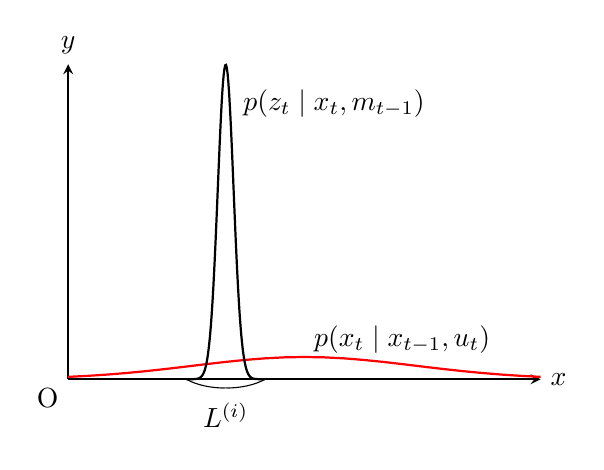
\begin{tikzpicture}
    % X Axis
    \draw[->,>=stealth,semithick] (0, 0) -- (6, 0) node[right]{$x$};
    % Y Axis
    \draw[->,>=stealth,semithick] (0, 0) -- (0, 4) node[above]{$y$};
    % Origin
    \draw (0, 0) node[below left]{O};

    % Motion Model Function
    \draw[red, thick, domain=0:6] plot(\x, {exp(-(\x - 3) * (\x - 3) / 2 / 2.0) / sqrt(2*pi*2.0)}) node[right]{};
    % Measurement Model Function
    \draw[thick, domain=1.5:2.5, samples=100] plot(\x, {exp(-(\x - 2) * (\x - 2) / 2 / 0.01) / sqrt(2*pi*0.01)}) node[right]{};
    
    \draw (2.1, 3.5) node[right]{$p(z_{t} \mid \bm{x}_{t}, m_{t-1})$};
    \draw (3, 0.5) node[right]{$p(\bm{x}_{t} \mid \bm{x}_{t-1}, u_{t})$};

    \draw [bend right, distance=0.3cm] (1.5, 0) to node[fill=white, inner sep=0.2pt, circle, below] {$L^{(i)}$} (2.5, 0);
   \end{tikzpicture}
   \caption{The Meaningful Area of the Observation Likelihood}
   \label{fig:meaningful_area_of_likelihood}
\end{figure}

このとき,オドメトリ動作モデルによってばらまかれたパーティクルの内,図\ref{fig:meaningful_area_of_likelihood}に示す観測モデルの意味のある領域$L^{(i)}$をカバーするパーティクルの数は非常に少なくなってしまいます.
$L^{(i)}$を十分な数のパーティクルで近似するには,以下の3つの対策が考えられます.

\begin{enumerate}
  \item 計算に使用するパーティクルの数を増やす
  \item 観測モデルを平滑化して分散を大きくし,$L^{(i)}$を無理やり大きくする
  \item パーティクルを観測に近い方向にばらまく
\end{enumerate}

パーティクルの数を増やせば当然$L^{(i)}$をカバーするパーティクルの数も増えますが,無駄な計算も多くなります.
観測モデルを平滑化して精度を落とせば$L^{(i)}$に近いパーティクルの重みをある程度確保できますが,せっかくのセンサのデータを破棄することにつながります.

というわけで,パーティクルを観測に近い方向にばらまくような提案分布を作れば良いということになります.
GMappingでは提案分布に観測の情報を統合することにより,観測モデルの意味のある領域にパーティクルを集中させる方法を取っています.
すなわち,

\begin{equation}
  p(\bm{x}_{t} \mid m_{t-1}^{(i)}, \bm{x}_{t-1}^{(i)}, z_{t}, u_{t})
  = \frac{p(z_{t} \mid m_{t-1}^{(i)}, \bm{x}_{t})p(\bm{x}_{t} \mid \bm{x}_{t-1}^{(i)}, u_{t-1})}{p(z_{t} \mid m_{t-1}^{(i)}, \bm{x}_{t-1}^{(i)}, u_{t})}
  \label{eq:improved_proposal}
\end{equation}

\noindent
を提案分布として使用します.
式\ref{eq:improved_proposal}を提案分布として使用したとき,パーティクルの重みの計算式は,

\begin{equation}
  \begin{split}
    w_{t}^{(i)} &= \eta \frac{p(z_{1:t} \mid \bm{x}_{t}^{(i)}, m_{t-1}^{(i)}) p(\bm{x}_{t}^{(i)} \mid \bm{x}_{t-1}^{(i)}, u_{t})}{p(\bm{x}_{t} \mid m_{t-1}^{(i)}, \bm{x}_{t-1}^{(i)}, z_{t}, u_{t})) w_{t-1}^{(i)}} \\
    &= \eta \frac{p(z_{1:t} \mid \bm{x}_{t}^{(i)}, m_{t-1}^{(i)}) p(\bm{x}_{t}^{(i)} \mid \bm{x}_{t-1}^{(i)}, u_{t})}{\frac{p(z_{t} \mid m_{t-1}^{(i)}, \bm{x}_{t})p(\bm{x}_{t} \mid \bm{x}_{t-1}^{(i)}, u_{t-1})}{p(z_{t} \mid m_{t-1}^{(i)}, \bm{x}_{t-1}^{(i)}, u_{t})}} \\
    &= \eta p(z_{t} \mid m_{t-1}^{(i)}, \bm{x}_{t-1}^{(i)}, u_{t})w_{t-1}^{(i)} \\
    &= \int p(z_{t} \mid \bm{x}^{\prime})p(\bm{x}^{\prime} \mid \bm{x}_{t-1}^{(i)}, u_{t})d\bm{x}^{\prime} \cdot w_{t-1}^{(i)}
  \end{split}
\end{equation}

\noindent
となります.
特徴ベースのFastSLAM2.0では,この改善された提案分布をガウス分布に近似したものを使用しています.
ランドマークの計測誤差がガウス分布に従うと仮定し,提案分布をカルマンフィルタによってガウス分布に近似します.
一方,GMappingのように占有格子地図を扱うSLAMでは,観測モデルの形状が予想できないため,特徴ベースのようにカルマンフィルタを使って近似するといったことができません.
そこで,GMappingではスキャンマッチングを用いて,状態遷移モデルによってばらまいたパーティクルを尤もらしい位置に補正しています.

まず,状態遷移モデルに従ってパーティクルを遷移させます.
この作業はFastSLAM1.0と変わりません.
次に,センサによって得られた観測情報を使って,状態遷移モデルで移動させたパーティクルを,尤度が高くなる位置に移動させます.
スキャンマッチングを適用した後,分布のガウス近似の中心と分散を求めます.
中心$\mu_{t}^{(i)}$と分散$\Sigma_{t}^{(i)}$の計算式は式\ref{eq:mean_and_covariance}となります.

\begin{equation}
  \begin{cases}
    \mu_{t}^{(i)} = \frac{1}{\eta^{(i)}} \sum_{j = 1}^{K} \bm{x}_{j} \cdot p(z_{t} \mid m_{t-1}^{(i)}, \bm{x}_{j}) \cdot p(\bm{x}_{j} \mid \bm{x}_{t-1}^{(i)}, u_{t}) \\
    \Sigma_{t}^{(i)} = \frac{1}{\eta^{(i)}} \sum_{j = 1}^{K}\bm{x}_{j} \mid m_{t-1}^{(i)}, \bm{x}_{j}) \cdot p(\bm{x}_{j} \mid \bm{x}_{t-1}^{(i)}, u_{t}) \cdot (\bm{x}_{j} - \mu_{t}^{(i)})(\bm{x}_{j} - \mu_{t}^{(i)})^{T}
  \end{cases}
  \label{eq:mean_and_covariance}
\end{equation}

\noindent
ここで,$\eta^{(i)}$は正規化因子で,式\ref{eq:normalized_factor}で計算できます.

\begin{equation}
  \eta^{(i)} = \sum_{j=1}^{K} p(z_{t} \mid m_{t-1}^{(i)}, \bm{x}_{j}) p(\bm{x}_{j} \mid \bm{x}_{t-1}^{(i)}, u_{t})
  \label{eq:normalized_factor}
\end{equation}

このようにすることで,改善された提案分布を求めることができるようになります.
従って,重みの計算式は式\ref{eq:particle_weight_by_improved_proposal}となります.

\begin{equation}
  \begin{split}
    w_{t}^{(i)} &= p(z_{t} \mid m_{t-1}^{(i)}, \bm{x}_{t-1}^{(i)}, u_{t}) w_{t-1}^{(i)} \\
    &= \int p(z_{t} \mid m_{t-1}^{(i)}, \bm{x}^{\prime})p(\bm{x}^{\prime} \mid \bm{x}_{t-1}^{(i)}, u_{t})d\bm{x}^{\prime} w_{t-1}^{(i)}\\
    &\simeq \sum_{j=1}^{K} p(z_{t} \mid m_{t-1}^{(i)}, \bm{x}_{j}) p(\bm{x}_{j} \mid \bm{x}_{t-1}^{(i)}, u_{t}) w_{t-1}^{(i)} \\
    &= \eta^{(i)} w_{t-1}^{(i)}
  \end{split}
  \label{eq:particle_weight_by_improved_proposal}
\end{equation}

実際に計算を行う際は,観測モデル$p(z_{t} \mid \bm{x}_{t}, m_{t-1}^{(i)})$はレーザービームの尤度場モデルが,状態遷移モデル$p(\bm{x}_{t} \mid \bm{x}_{t-1}, u_{t})$にはオドメトリ動作モデルが使われます.
オドメトリ動作モデルは\ref{sec:motion_model_odometry}で,尤度場モデルは\ref{sec:likelihood_field_model}で説明します.

\subsection{リサンプリングアルゴリズム}

GMappingでは,パーティクルをリサンプリングするタイミングを決めるための指標として,式\ref{eq:adaptive_resampling}に示す$N_{\text{eff}}$という数値を導入しています.

\begin{equation}
  N_{\text{eff}} = \frac{1}{\sum_{i=1}^{N} (\tilde{w_{(i)}})^2}
  \label{eq:adaptive_resampling}
\end{equation}

$N$はパーティクルの数です.
$N_{\text{eff}}$は現在のパーティクルが事後分布をどれだけよく表しているかを示す指標で,正規化されたパーティクルの重み$\tilde{w_{(i)}}$の2乗和の逆数で計算されます.

$N_{\text{eff}}$の直観的理解は以下のようなものです:
もしパーティクルが事後分布から引き出された場合,importance samplingの原理により,それらの重みは互いに等しくなります.
逆に,パーティクルによる事後分布の近似の精度が悪いと,パーティクルの重みの分散は大きくなります.
言い換えれば,$N_{\text{eff}}$はパーティクルの重みの分散の尺度とみなすことができるため,パーティクルの集合が事後分布をどれだけ近似しているかを評価する尺度として利用することができます.

パーティクルの重みがすべて等しいとき,$N_{\text{eff}}$の値は$N^2$に等しくなります.
逆に各パーティクルの重みの差が大きくなると,$N_{\text{eff}}$の値は1に近づきます.

GMappingでは,$N_{\text{eff}}$が閾値$\frac{N}{2}$を下回ったときにリサンプリングが実行されます.\cite{Gmapping}
数式で表すと式\ref{eq:neff}のようになります.

\begin{equation}
  N_{\text{eff}} < \frac{N}{2}
  \label{eq:neff}
\end{equation}

ROSの\textsf{slam\_gmapping}では,このリサンプリングの閾値は\textsf{resampleThreshold}で決定することができます.
これは$\frac{N_{\text{eff}}}{N}$の比の閾値として定義されており,デフォルト値は0.5に設定されています.
すなわち,

\begin{equation}
  \frac{N_{\text{eff}}}{N} < \textsf{resampleThreshold} = 0.5 \text{(default)}
  \label{eq:neff_ros}
\end{equation}

\noindent
という条件を満たしたとき,リサンプリングが行われるようになります.

\subsection{オドメトリ状態遷移モデル}
\label{sec:motion_model_odometry}

ここではホイールオドメトリによって状態遷移モデル$p(\bm{x}_{t} \mid \bm{x}_{t-1}, u_{t})$を求める手順を説明します.
オドメトリによって求めた時刻$t$のロボットの姿勢を$\bar{\bm{x}}_{t}$と表記することにします.
ホイールオドメトリはドリフトやスリップによる誤差を含むので,オドメトリ座標系でのロボットの姿勢$\bar{\bm{x}_{t}}$とグローバル座標系でのロボットの姿勢$\bm{x}_{t}$は一致することはありません.

一方で,$\bar{\bm{x}}_{t-1}$から$\bar{\bm{x}}_{t}$までの相対的な移動量の差分は,真の姿勢$\bm{x}_{t-1}$から$\bm{x}_{t}$との差分とそれほどズレているわけではないため,いい感じの推定量として使用することができます.
そこで,ロボットの移動の情報$u_{t}$を式\ref{eq:motion_information}のように定義することにします.

\begin{equation}
  u_{t} =
  \begin{pmatrix}
    \bar{\bm{x}}_{t-1} \\
    \bar{\bm{x}}_{t}
  \end{pmatrix}
  \label{eq:motion_information}
\end{equation}

そして,$u_{t}$を更に3つのパラメータ$\delta_{\text{rot}1}$,$\delta_{\text{trans}}$,$\delta_{\text{rot}2}$に分解して考えます.
$\delta_{\text{rot}1}$,$\delta_{\text{trans}}$,$\delta_{\text{rot}2}$は移動量を表す変数で,これを使うことにより,$u_{t}$は以下のような3段階のシーケンスで表されます.

\begin{itemize}
  \item 回転量$\delta_{\text{rot}1}$だけ旋回
  \item 並進量$\delta_{\text{trans}}$だけ並進
  \item 回転量$\delta_{\text{rot}2}$だけ旋回
\end{itemize}

\begin{figure}[ht]
  \centering
  \begin{tikzpicture}
    % Body t-1
    \draw[thick, rotate around={-105:(0, 0)}]
      (0, 0.5) -- (0.5, 0.25) -- (0.5, -0.5)
        -- (-0.5, -0.5) -- (-0.5, 0.25) -- (0, 0.5);
    \draw[rotate around={30:(0, 0)}] (0, 0) -- (6, 0);
    % Body t
    \draw[thick, rotate around={75:(5.2, 3)}]
    (5.7, 3) -- (5.45, 2.5) -- (4.7, 2.5)
      -- (4.7, 3.5) -- (5.45, 3.5) -- (5.7, 3);

    \draw[rotate around={-15:(0, 0)}] (0, 0) -- (1, 0);
    \draw[rotate around={30:(5.2, 3)}] (5.2, 3) -- (6.2, 3);
    \draw[rotate around={75:(5.2, 3)}] (5.2, 3) -- (6.2, 3);

    \draw[rotate around={-15:(0, 0)}] (0.8, 0) arc [start angle=0, delta angle=45, radius=0.8];
    \draw[rotate around={30:(5.2, 3)}] (6, 3) arc [start angle=0, delta angle=45, radius=0.8];

    \draw (3, 2) node[above]{$\delta_{\text{trans}}$};
    \draw (0.8, 0.2) node[right]{$\delta_{\text{rot1}}$};
    \draw (5.6, 3.6) node[above right]{$\delta_{\text{rot2}}$};

    \draw (0, 0.6) node[above]{$\bm{x}_{t-1}$};
    \draw (5.2, 2) node[above]{$\bm{x}_{t}$};
  \end{tikzpicture}
  \caption{Three Parameters of the Odometry Motion Model}
  \label{fig:three_parameters_of_the_odometry_motion_model}
\end{figure}

言い換えれば,姿勢のペア$(\bar{\bm{x}}_{t-1}, \bar{\bm{x}}_{t})$はパラメータとして要素数3のベクトル$(\delta_{\text{rot}1}, \delta_{\text{trans}}, \delta_{\text{rot}2})^{T}$を持ち,このベクトルは$(\bar{\bm{x}}_{t-1}, \bar{\bm{x}}_{t})$を再構築するのに十分な情報を持っていることになります.
というわけで,このベクトルをオドメトリの情報として使用することにします.

これらのパラメータ$\delta_{\text{rot}1}$,$\delta_{\text{trans}}$,$\delta_{\text{rot}2}$はそれぞれ独立したノイズを持つと仮定すると,状態遷移モデル$p(\bm{x}_{t} \mid \bm{x}_{t-1}, u_{t})$を計算するアルゴリズムはアルゴリズム\ref{alg:motion_model_odometry}のようになります.

\begin{algorithm}
  \caption{motion\_model\_odometry}
  \label{alg:motion_model_odometry}
  \begin{algorithmic}[1]
    \REQUIRE $\bm{x}_{t} = (x_{t}, y_{t}, \theta_{t})^{T}, \bm{x}_{t-1} = (x_{t-1}, y_{t-1}, \theta_{t-1})^{T}, u_{t} = (\bar{\bm{x}}_{t-1}, \bar{\bm{x}}_{t})^{T}$
    \ENSURE $p(\bm{x}_{t} \mid \bm{x}_{t-1}, u_{t})$

    \STATE $\delta_{\text{rot1}} = \text{atan2}(\bar{y}_{t} - \bar{y}_{t-1}, \bar{x}_{t} - \bar{x}_{t-1}) - \bar{\theta}_{t-1}$
    \STATE $\delta_{\text{trans}} = \sqrt{(\bar{x}_{t-1} - \bar{x}_{t})^2 + (\bar{y}_{t-1} - \bar{y}_{t})^2}$
    \STATE $\delta_{\text{rot2}} = \bar{\theta}_{t} - \bar{\theta}_{t-1} - \delta_{\text{rot1}}$

    \STATE $\hat{\delta}_{\text{rot1}} = \text{atan2}(y_{t} - y_{t-1}, x_{t} - x_{t-1}) - \theta_{t-1}$
    \STATE $\hat{\delta}_{\text{trans}} = \sqrt{(x_{t-1} - x_{t})^2 + (y_{t-1} - y_{t})^2}$
    \STATE $\hat{\delta}_{\text{rot2}} = \theta_{t} - \theta_{t-1} - \hat{\delta}_{\text{rot1}}$

    \STATE $p_1 = \text{prob}(\delta_{\text{rot1}} - \hat{\delta}_{\text{rot1}}, \alpha_1 \hat{\delta}_{\text{rot1}} + \alpha_2 \hat{\delta}_{\text{trans}})$
    \STATE $p_2 = \text{prob}(\delta_{\text{trans}} - \hat{\delta}_{\text{trans}}, \alpha_3 \hat{\delta}_{\text{trans}} + \alpha_4 (\hat{\delta}_{\text{rot1}} + \hat{\delta}_{\text{rot2}}))$
    \STATE $p_3 = \text{prob}(\delta_{\text{rot2}} - \hat{\delta}_{\text{rot2}}, \alpha_1 \hat{\delta}_{\text{rot2}} + \alpha_2 \hat{\delta}_{\text{trans}})$

    \STATE return $p_1 \cdot p_2 \cdot p_3$
  \end{algorithmic}
\end{algorithm}

尚,アルゴリズム\ref{alg:motion_model_odometry}における$\text{prob}(a, b)$関数は,平均$a$,分散$b$の確率分布(ガウス分布もしくは三角分布)を表します.

実際にパーティクルフィルタを実装する場合は,アルゴリズム\ref{alg:motion_model_odometry}を使って確率分布そのものを求めるよりも,その分布から姿勢をドローした結果を求めるのが一般的です.
アルゴリズム\ref{alg:sample_motion_model_odometry}がそのアルゴリズムの実装例です.

\begin{algorithm}
  \caption{sample\_motion\_model\_odometry}
  \label{alg:sample_motion_model_odometry}
  \begin{algorithmic}[1]
    \REQUIRE $\bm{x}_{t-1} = (x_{t-1}, y_{t-1}, \theta_{t-1})^{T}, u_{t} = (\bar{\bm{x}}_{t-1}, \bar{\bm{x}}_{t})^{T}$
    \ENSURE $\bm{x}_{t} = (x_{t}, y_{t}, \theta_{t})^{T}$ sampled from $p(\bm{x}_{t} \mid \bm{x}_{t-1}, u_{t})$

    \STATE $\delta_{\text{rot1}} = \text{atan2}(\bar{y}_{t} - \bar{y}_{t-1}, \bar{x}_{t} - \bar{x}_{t-1}) - \bar{\theta}_{t-1}$
    \STATE $\delta_{\text{trans}} = \sqrt{(\bar{x}_{t-1} - \bar{x}_{t})^2 + (\bar{y}_{t-1} - \bar{y}_{t})^2}$
    \STATE $\delta_{\text{rot2}} = \bar{\theta}_{t} - \bar{\theta}_{t-1} - \delta_{\text{rot1}}$

    \STATE $\hat{\delta}_{\text{rot1}} = \delta_{\text{rot1}} - \text{sample}(\alpha_1 \delta_{\text{rot1}} + \alpha_2 \delta_{trans})$
    \STATE $\hat{\delta}_{\text{trans}} = \delta_{\text{trans}} - \text{sample}(\alpha_3 \delta_{\text{trans}} + \alpha_4(\delta_{\text{rot1}} + \delta_{\text{rot2}}))$
    \STATE $\hat{\delta}_{\text{rot2}} = \delta_{\text{rot2}} - \text{sample}(\alpha_1 \delta_{\text{rot2}} + \alpha_2 \delta_{\text{trans}})$

    \STATE $x_{t} = x_{t-1} + \hat{\delta}_{\text{trans}} \cos(\theta_{t-1} + \hat{\delta}_{\text{rot1}})$
    \STATE $y_{t} = y_{t-1} + \hat{\delta}_{\text{trans}} \sin(\theta_{t-1} + \hat{\delta}_{\text{rot1}})$
    \STATE $\theta_{t} = \theta_{t-1} + \hat{\delta}_{\text{rot1}} + \hat{\delta}_{\text{rot2}}$

    \STATE return $\bm{x}_{t} = (x_{t}, y_{t}, \theta_{t})^T$
  \end{algorithmic}
\end{algorithm}

ここで,$\text{sample}(b)$は分散$b$の分布(ガウス分布または三角分布)からノイズをドローする関数です.
アルゴリズム\ref{alg:sample_motion_model_odometry}は,入力として$\bm{x}_{t-1}$と$u_{t}$を受け取り,出力として$p(\bm{x}_{t} \mid \bm{x}_{t-1}, u_{t})$に従うランダムな$\bm{x}_{t}$を返します.
確率分布そのものを求めるよりも簡単に計算でき,ドローした姿勢をすぐに計算に使うことができるので,プログラムとして実装する際はこちらのアルゴリズムが使用されます.

\subsection{レーザービームの尤度場モデル}
\label{sec:likelihood_field_model}

GMappingでは観測モデルとしてレーザービームの尤度場モデル(\textsf{likelihood\_field\_model})が使われています.
尤度場モデルは距離センサの確率モデルの1つで,もっともらしい物理的な証明のないアドホックなモデルですが,良く機能するモデルとされています.

尤度場モデルのキーアイデアは,レーザースキャンの各ビームの終点をグローバル座標に投影して計算を行うことにあります.
グローバル座標系における時刻$t$のロボットの姿勢を$\bm{x}_{t} = (x_{t}, y_{t}, \theta_{t})^T$,ロボット座標系でのセンサの位置を$(x_{k, \text{sens}}, y_{k, \text{sens}})^T$,センサから見たビームの角度を$\theta_{k, \text{sens}}$,距離を$z_{t}^{k}$とすると,ビームの終点のグローバル座標は式\ref{eq:beam_endpoint_transform}で表されます.

\begin{equation}
  \begin{pmatrix}
    x_{z_{t}^{k}} \\
    y_{z_{t}^{k}}
  \end{pmatrix}
  =
  \begin{pmatrix}
    x_{t} \\
    y_{t}
  \end{pmatrix}
  +
  \begin{pmatrix}
    \cos{\theta_{t}} & -\sin{\theta_{t}} \\
    \sin{\theta_{t}} & \cos{\theta_{t}}
  \end{pmatrix}
  \begin{pmatrix}
    x_{k, \text{sens}} \\
    y_{k, \text{sens}}
  \end{pmatrix}
  + z_{t}^{k}
  \begin{pmatrix}
    \cos{\theta_{t} + \theta_{k, \text{sens}}} \\
    \sin{\theta_{t} + \theta_{k, \text{sens}}} \\
  \end{pmatrix}
  \label{eq:beam_endpoint_transform}
\end{equation}

この座標変換の関係を図で表したのが図\ref{fig:beam_endpiont_transoform}です.
図\ref{fig:beam_endpoint_transform}ではグローバル座標系とオドメトリ座標系がかなり離れているように見えますが,オドメトリの精度によってはそれほど乖離することはありません.

\begin{figure}[ht]
  \centering
  \begin{tikzpicture}
    % Global Coordinate Axis
    \draw (0, 0) node[below]{$\Sigma_{\text{map}}$};
    \draw[->, >=stealth, semithick] (0, 0) -- (1.5, 0) node[right]{$x$};
    \draw[->, >=stealth, semithick] (0, 0) -- (0, 1.5) node[above]{$y$};

    % Odometry Coordinate Axis
    \draw (2, 1) node[below]{$\Sigma_{\text{odom}}$};
    \draw[->, >=stealth, semithick, rotate around={30:(2, 1)}] (2, 1) -- (3.5, 1) node[right]{$x$};
    \draw[->, >=stealth, semithick, rotate around={30:(2, 1)}] (2, 1) -- (2, 2.5) node[above]{$y$};

    % Robot
    \draw[rotate around={45:(4, 3)}] (4, 3) -- (3.75, 3.5) -- (3, 3.5) -- (3, 2.5) -- (3.75, 2.5) -- (4, 3);
    \draw[->, >=stealth, semithick, rotate around={45:(4, 3)}] (3.5, 3) -- (4, 3);
    \draw[->, >=stealth, semithick, rotate around={45:(4, 3)}] (3.5, 3) -- (3.5, 3.5);
    
    % Sensor
    \draw[->, >=stealth, semithick, blue, rotate around={45:(4, 3)}] (4, 3) -- (4.5, 3);
    \draw[->, >=stealth, semithick, blue, rotate around={45:(4, 3)}] (4, 3) -- (4, 3.5);

    % Beam
    \draw[blue, dotted, rotate around={45:(4, 3)}] (4, 3) -- (5.73, 4);
    \fill (4.517, 4.932) circle [blue, radius=2pt];
    \draw[blue, rotate around={45:(4, 3)}] (4, 3) -- (6, 3);
    \draw[thick, ->, rotate around={45:(4, 3)}] (5, 3) arc [start angle=0, delta angle=30, radius=1];
    \draw (4.5, 5) node[above]{$(x_{z_{t}^{k}}, y_{z_{t}^{k}})^T$};
    \draw (4.5, 3.5) node[right]{$\theta_{k, \text{sens}}$};
  \end{tikzpicture}
  \caption{Beam Endpoint Transform}
  \label{fig:beam_endpiont_transoform}
\end{figure}

この座標変換は,センサが障害物を検知したときのみ意味を持ちます.
センサが障害物を検知できなかったとき,一般的に,距離センサは最大測定範囲の数値を返します.
センサが最大値を返したとき,式\ref{eq:beam_endpoint_transform}の座標変換は,物理空間において意味を持たなくなります.
尤度場モデルにおいて,センサが最大値を返したときは単純にその値を無視します.

尤度場モデルは以下に示す3つのノイズを考慮します.

\begin{enumerate}
  \item 測定ノイズ$p_{\text{hit}}$ \\
  距離センサによって障害物までの距離を測定するときに混入する偶然誤差です.
  誤差の大きさはガウス分布によって近似することができます.
  
  ビームの終点座標$(x_{z_{t}^k}, y_{z_{t}^k})^T$と,それに一番近い地図$m_[t-1]$の障害物(占有格子地図では障害物セル)とのユークリッド距離を$\text{dist}$という変数で置くと,このノイズの確率モデルは式\ref{eq:p_hit}で表されます.
  $\epsilon_{\sigma_{\text{hit}}^{2}}(x)$は平均0,分散$\sigma_{\text{hit}}^2$のガウス分布です.
  
  \begin{equation}
    p_{\text{hit}}(z_{t}^{k} \mid \bm{x}_{t}, m_{t-1}) = \epsilon_{\sigma_{\text{hit}}^{2}}(\text{dist}^2) = \frac{1}{\sqrt{2\pi \sigma_{\text{hit}}^2}} \exp\left(-\frac{\text{dist}^2}{2\sigma_{\text{hit}}^2}\right)
    \label{eq:p_hit}
  \end{equation}
  
  \noindent
  で表されます.
  
  ガウス分布に$\text{dist}$を代入したときの値が,そのビームの観測尤度となります.
  障害物との距離が0のとき,すなわち観測誤差が0のとき,そのビームの尤度は最大になります.
  \item 計測失敗$p_{\text{max}}$ \\
  センサが最大測定範囲の値を返したとき,測定失敗とみなします.
  この誤差は極小幅の一様分布としてモデリングします.
  \item ランダム測定$p_{\text{rand}}$ \\
  一様に出現する原因不能なノイズをランダム測定として定義します.
  この分布は一様分布でモデル化します.
\end{enumerate}

ビーム一本の観測モデルは,これらのモデルを線形結合したものになります.

\begin{equation}
  p(z_{t}^{k} \mid \bm{x}_{t}, m_{t-1}) = z_{\text{hit}} \cdot p_{\text{hit}} + z_{\text{rand}} \cdot p_{\text{rand}} + z_{\text{max}} \cdot p_{\text{max}}
  \label{eq:beam_likelihood}
\end{equation}

ただし,$z_{\text{hit}}$,$z_{\text{rand}}$,$z_{\text{max}}$は各分布の重みづけ係数で,$z_{\text{hit}} + z_{\text{rand}} + z_{\text{max}} = 1$です.

GMappingでは$p_{\text{max}}$は扱っていないようなので,\footnote{ソースコードを見てそう判断しました.実際そうなっているかどうかの証拠は見つかっていません.}
ビームの観測モデルは式\ref{eq:beam_likelihood_im_gmapping}のようになっていると思われます.

\begin{equation}
  p(z_{t}^{k} \mid \bm{x}_{t}, m_{t-1}) = (1 - z_{\text{rand}}) \cdot p_{\text{hit}} + z_{\text{rand}}
  \label{eq:beam_likelihood_im_gmapping}
\end{equation}

一度のレーザースキャンにおいて,各ビームの測定誤差がそれぞれ独立していると仮定すると,レーザースキャン$z_{t}$の尤度は式\ref{eq:measurement_model}のように計算できます.

\begin{equation}
  p(z_{t} \mid \bm{x}_{t}, m_[t-1]) = \prod_{j=0}^{K-1} p(z_{t}^{j} \mid \bm{x}_{t}, m_{t-1})
  \label{eq:measurement_model}
\end{equation}

式\ref{eq:measurement_model}には指数の計算が含まれる他,少数の掛け算を何度も繰り返すので,このままプログラムとして実装するのはあまりよろしくありません.
GMappingでは尤度関数の自然対数を取り,乗算を加算として計算しているようです.
\footnote{\url{https://github.com/ros-perception/openslam_gmapping/blob/6b9b23bf2a7ad7c04a33c6f52371c5621ffe613e/include/gmapping/scanmatcher/scanmatcher.h\#L243}}

\end{document}